\documentclass[11pt, singlecolumn, citestyle=authoryear]{elegantbook}
\definecolor{customcolor}{RGB}{153,204,255}
\colorlet{coverlinecolor}{customcolor}
\usepackage{wrapfig}
\usepackage{lmodern}
\usepackage{lipsum,graphicx}
\usepackage[utf8]{inputenc} %unicode support
\usepackage[T1]{fontenc}


\newcommand{\compresslist}{%
	\setlength{\itemsep}{0pt}%
	\setlength{\parskip}{1pt}%
	\setlength{\parsep}{0pt}%
}


\title{FUTURE-DATA\\Dublin Bikes}
\date{Due: April 21, 2023}
\author{Ariana Alves Antunes, Imelda Finn, Marcus Ò Faolain}

\begin{document}
	\mainmatter 
	
\chapter*{FUTURE-DATA\\Dublin Bikes \\\ Ariana Alves Antunes, Imelda Finn, Marcus Ò Faolain}

 	\subsection*{Introduction}
This assignment is measuring the impact of pandemic on Dublin City Bikes within difference scenario. 
	

\section {The impact of the pandemic on bike usage}
%To assess the impact of the pandemic on the city-bike usage;
	Due to lockdonw and restrictions in Dublin during COVID,  bike usaged was directly impacted as shown in the figures below from 2019 and 2020, more people were choosing to cycle over public transportation. However with business closed and working from home, the usaged dropped by half. Just Eat dublin bikes latest summary statistics below as at 31/08/2019, current valid annual subscribers  was 66,940 with €25 membership fee, plus revenue made with advertising. 

	\begin{figure}[h!]
		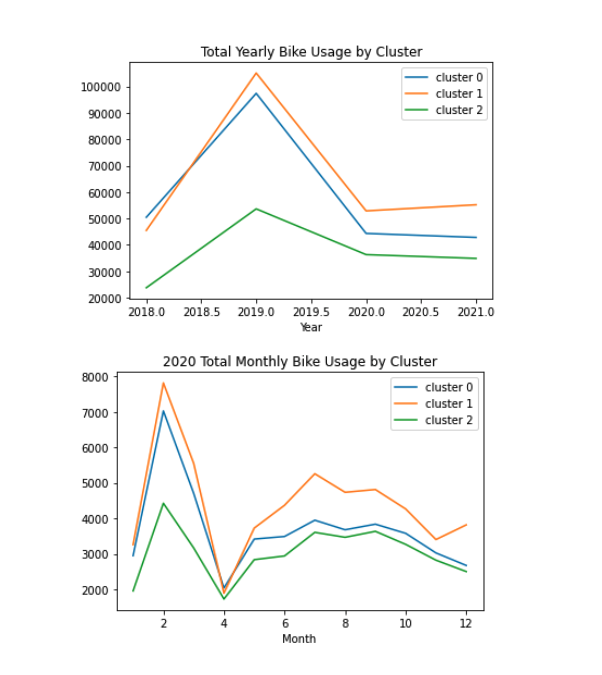
\includegraphics[width=0.7\textwidth]{../graphs/usaged_total_plus2020.png}
		\caption{Total bike usage and total usaged for 2020}
		\label{fig:surface}
	\end{figure}

As it can be observed with the graphs the constrast between before pandemic and  4 month after, there is a decline between full lockdown and when restrictions imposed by the Government were lifted. Since the bikes are membership payments on a yearly basis, the risk of not acquiring new clients could be a major risk for the business, still the essential works were a big part of the new audience being attracted to Dublin bikes. 

\begin{table}[h!]
	\begin{tabular}{|l|r|r|}
		Year & Usage \\
		2018 & 13464.0 \\
		2019 & 26501.0 \\ 
		2020 & 11106.0 \\ 
		2021 & 8188.0 \\ 
		
	\end{tabular} 
\end{table}

\begin{comment}
	\begin{figure}[!htbp]
		\includegraphics[width=0.7\textwidth]{graphs/q2_xy.png}
		\includegraphics[width=0.7\textwidth]{graphs/q2_hist.png}
		\caption{Q2 Data}
		\label{fig:mle}
	\end{figure}
\end{comment}


\section{Predicted bike usage for 2020}
%2. To estimate how the city-bike usage would have been without the pandemic (e.g., 2020) 

The bike usage was way down compared to the prediction.\footnote{RidgeCV(alphas=(0.1, 1.0, 10.0), cv=None, fit\_intercept=True, gcv\_mode=None, normalize=False, scoring=None, store\_cv\_values=False)}  
The prediction isn't too bad for January, February, but usage drops at the end of February and stays down for the rest of the year.
\begin{figure}[!htbp]
	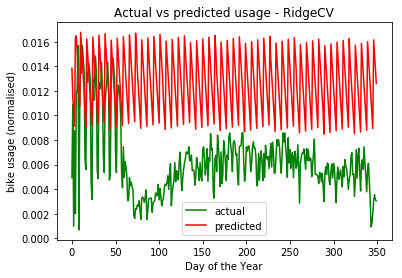
\includegraphics[width=0.7\textwidth]{../graphs/pred_2020.png}
	\caption{Predicted bike usage in 2020, compared to actual usage}
	\label{fig:surface}
\end{figure}

The pandemic also led to changes in cycling infrastructure in Dublin. The Dublin City Council implemented temporary measures, such as pop-up bike lanes and widened footpaths, to support cycling and promote social distancing. These measures were later made permanent, resulting in an increase in the number of dedicated cycle lanes across the city.

Overall, the pandemic has had a positive opportunity  on bike usage in Dublin, with more people choosing to cycle as a means of transport. The increased interest in cycling has led to improvements in cycling infrastructure and the creation of more cycling-friendly routes in the city.


%\section{Predicted bike usage for 2022} 
%To predict the city-bike usage for 2022 in both the pandemic and no-pandemic scenarios. Use both qualitative and quantitative comparisons.

	
\subsection*{Technical/Data issues}
There was some missing data for a few years, which was directly impacting the results, so it was removed. Assigned 2 stations from each cluster, the cluster 2 stations had similar pre-pandemic characteristics and both serve hospitals. Excluded stations with less than 300,000 data points.   None of the stations were open the whole time. The variable modelled is usage, which is the absolute difference in available bikes from one time point to the next.  For modelling, this is normalised by dividing by the number of bike stands.



\begin{table}[h]
	\begin{tabular}{|l|r|r|}
		Station Name & cluster & bike stands\\
		FITZWILLIAM SQUARE EAST & 0 & 40\\
		HANOVER QUAY & 0 & 40\\
		MATER HOSPITAL & 2 & 40\\
		NEW CENTRAL BANK & 1 & 40 \\
		PARNELL SQUARE NORTH & 2 & 20\\
		YORK STREET EAST & 1 & 32 \\
		
	\end{tabular} 
\end{table}

\begin{figure}[h!]
	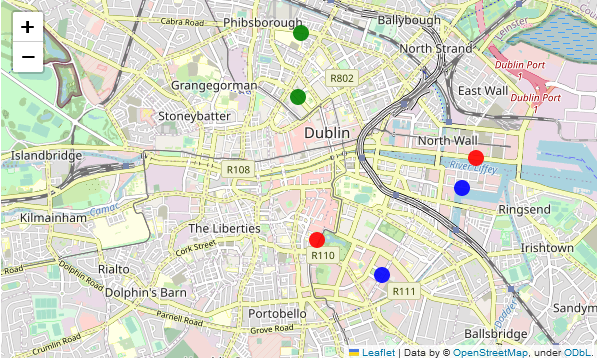
\includegraphics[width=0.5\textwidth]{../graphs/bikeStationMap.png}
	\caption{Selected Bike Stations}
	\label{fig:stations}
\end{figure}


\section*{Code Reference}

\texttt{https://github.com/Arianaxsz/ML-Project}

Code in \texttt{fileName.ipynb}, \texttt{py/fileName.py}

\texttt{Pre-processing: dublin$_$bike$_$analysis.ipynb}

\texttt{Model: model$_$q2.ipynb}

\texttt{Data Visualization: Usage graphs.ipynb}

%===============================================================

% # Code snippets

%\vspace{.25cm}
%\noindent  %\href{https://www.researchgate.net/profile/Adam_Przeworski/publication/240357392_Classifying_Political_Regimes/links/0deec532194849aefa000000/Classifying-Political-Regimes.pdf}{Alvarez, Cheibub, Limongi, and Przeworski (1996)}


%\input{tables/zip_poisson.tex}

\begin{comment}
	
	\begin{figure}[!htbp]
		\includegraphics[width=0.7\textwidth]{graphics/wireframe.pdf}
		\caption{mle surface}
		\label{fig:surface}
	\end{figure}
	\begin{figure}[!htbp]
		\includegraphics[width=0.7\textwidth]{graphics/q2_xy.png}
		\includegraphics[width=0.7\textwidth]{graphics/q2_hist.png}
		\caption{Q2 Data}
		\label{fig:mle}
	\end{figure}
\end{comment}

\begin{comment}
	\begin{sidewaystable}
		%\begin{tabular}...\end{tabular}
	\end{sidewaystable}
	%\input{tables/gdp_crosstab.tex}
	
	\begin{landscape}
		\include{tables/gdp_crosstab.tex}
	\end{landscape}
	
\end{comment}


\end{document}
